\section{Component segment coordinate transform}
%
\begin{figure}[htb]
  \centering
  % trim left, bottom, right , top
  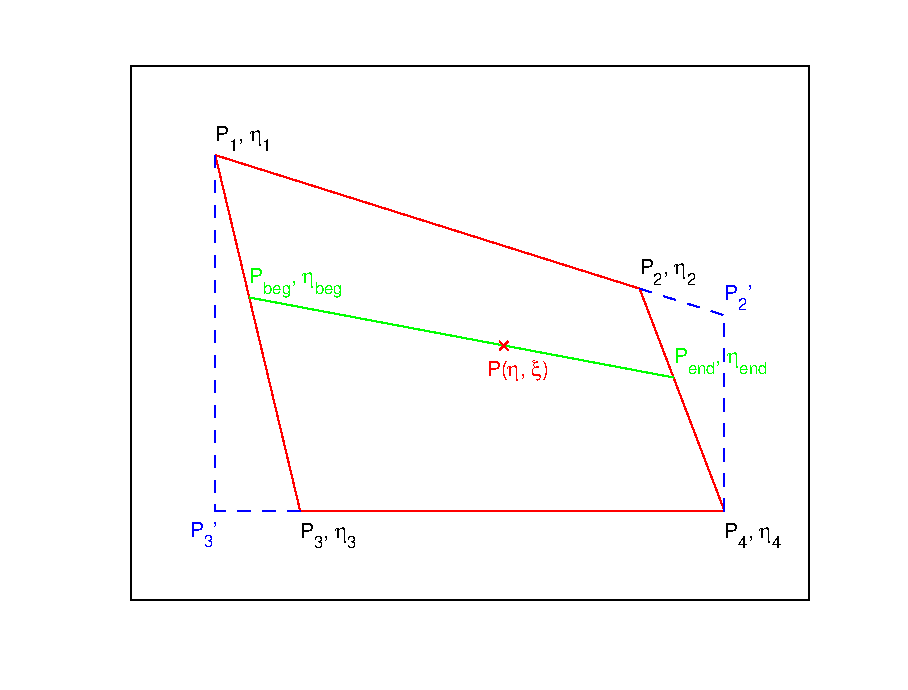
\includegraphics[trim=1cm 1cm 1cm 0.5cm, clip=true,width = 8cm]{gfx/compSegTheo}
	\caption{Illustration for the calculation of the component segment coordinate transformation}
	\label{fig:cs_surf}
\end{figure}
%
The coordinate transform of component segment coordinates is somewhat more complicated than the segment coordinate transform. To simplify the procedure, the component segment should consist of only one segment for now. The segment is again defined by its corner points $\vec p_1 \dots \vec p_4$. Figure \ref{fig:cs_surf} should help understanding the forthcoming calculations. \par
First we need some definitions:
\begin{itemize}
	\item Leading edge:  $ \vec s_v = \vec p_2 - \vec p_1 $
	\item Trailing edge: $ \vec s_h = \vec p_4 - \vec p_3 $
	\item Projected leading edge:   $\vec n = -\vec s_v$, with $n_x = 0$  
\end{itemize}


\subsection{Extending leading and trailing edges}
Plane through $\vec p_4$ with normal vector $\vec n$. Calculate inersection with leading edge. Plane equation is:
\begin{equation}
(\vec p - \vec p_4) \cdot \vec n = 0
\label{eq:plane}
\end{equation}
 Linear equation for the leading edge:
 
\begin{equation}
\vec p = \vec p_1 + \alpha (\vec p_2 - \vec p_1)
\label{eq:lin_eq1}
\end{equation}

Inserting (\ref{eq:lin_eq1}) into (\ref{eq:plane}) yields:
\begin{equation}
\alpha_v = \frac {(\vec p_4 - \vec p_1) \cdot \vec n }{(\vec p_2 - \vec p_1) \cdot \vec n}
\label{eq:nothing}
\end{equation}
%
If $\alpha_v > 1$, the leading edge has to be extended, else the trailing edge must be extended. In the first case, we calculate the extended leading edge point $\vec p_2^\prime$:
\begin{equation}
\vec p_2^\prime = \vec p_1 + \alpha_v (\vec p_2 - \vec p_1)
\label{eq:}
\end{equation}
%
In the other case ($\alpha_v < 1$), the intersection point with the trailing edge can be calculated in the same fashion.  \par
Now, we apply the same method also to the inner section, getting the extended points $\vec p_1^\prime$ and $\vec p_2^\prime$.

\subsection{Calculating $\eta$ values of the corners}
For the following calculations, we need to know the eta coordinates of the corner points $\vec p_1 \dots \vec p_4$. Lets image a plane with the previously defined normal vector $\vec n$ that goes through one of these points. Without loss of generality, let this point be $\vec p_3$. This plane is then defined by the equation
%
\begin{equation}
(\vec p - \vec p_3) \cdot \vec n = 0
\label{eq:plane_p3}
\end{equation}
%
Now we should find out, at which eta coordinate the plane intersects the leading edge, which is now parametrized as follows:
\begin{equation}
p = \vec p_1^ \prime + \eta ({\vec p_2}^\prime - {\vec p_1}^\prime).
\end{equation}
Combining both equations leads to $\eta_3 = \frac {(\vec p_3 - {\vec p_1}^\prime) \cdot \vec n }{({\vec p_2}^\prime - {\vec p_1}^\prime) \cdot \vec n}$, or in general:
\begin{equation}
\eta_i = \frac {(\vec p_i - {\vec p_1}^\prime) \cdot \vec n }{({\vec p_2}^\prime - {\vec p_1}^\prime)\cdot \vec n}.
\end{equation}

After doing these calculations (which have to be done only once), we can finally proceed to the coordinate transform.

\subsection{Calculating 3D coordinates of the $(\eta, \xi)$ pair}
The easiest way to do the transformation is to move first in $\xi$ direction. As the component segment is straight between the points $(\vec p_1, \vec p_3)$ and $(\vec p_2, \vec p_4)$ by definition, we move first along these lines:
\begin{align}
\vec p_{beg}(\xi) &= (1-\xi)\vec p_1 + \xi \vec p_3 \\
\vec p_{end}(\xi) &= (1-\xi)\vec p_2 + \xi \vec p_4
\end{align}

The corresponding eta coordinates of the points are 
\begin{align}
\eta_{beg}(\xi) &= (1-\xi)\eta_1 + \xi \eta_3 \\
\eta_{end}(\xi) &= (1-\xi)\eta_2 + \xi \eta_4
\end{align}

Finally, we walk along the line defined by the new point $\vec p_{beg}$ and $\vec p_{end}$ (depicted green in figure \ref{fig:cs_surf}). We have to keep in mind their eta coordinates (which are not 0 and 1)! We get our final result

\begin{equation}
\vec p(\eta, \xi) = \vec p_{beg} (\xi) + \frac {\eta - \eta_{beg}(\xi)}{\eta_{end}(\xi) - \eta_{beg}(\xi)} \cdot \left( \vec p_{end}(\xi) - \vec p_{beg}(\xi) \right).
\end{equation}